% 第 18 题三棱台：按固定源 PDF 矢量路径换算（1 pt → 0.03515 cm）。
% 原点取 A 点（源页 (237.39, 177.27) pt），y 向上。
% 上底面 D-E-F（D 左上、F 右上、E 居中略低）、下底面 A-B-C（A 左、C 右、B 下方）。
% 实线 10 条：侧棱 AD/EB/FC、上底 DF/DE/EF、下底 BA/BC、辅助线 DB（第 (2) 问所问直线）与侧面 BCFE 对角线 FB；
% 虚线 1 条：AC（被遮挡的下底棱，stroke-dasharray 直接判定）。各顶点旁标注 A/B/C/D/E/F（照源字形框中心）。
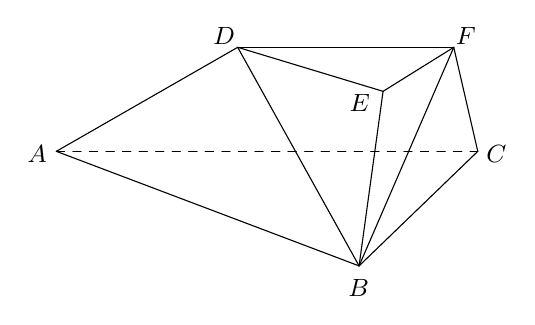
\begin{tikzpicture}[line cap=round,line join=round,font=\small,x=0.03515cm,y=0.03515cm]
\draw (0,0)--(65.52,37.58);             % A–D（侧棱）
\draw (65.52,37.58)--(143.57,37.58);    % D–F（上底棱，水平）
\draw (65.52,37.58)--(118.04,21.68);    % D–E（上底棱）
\draw (118.04,21.68)--(143.57,37.58);   % E–F（上底棱）
\draw (143.57,37.58)--(152.25,0);       % F–C（侧棱）
\draw (118.04,21.68)--(109.37,-41.38);  % E–B（侧棱）
\draw (65.52,37.58)--(109.37,-41.38);   % D–B（辅助线）
\draw (143.57,37.58)--(109.37,-41.38);  % F–B（侧面 BCFE 对角线）
\draw (0,0)--(109.37,-41.38);           % A–B（下底棱）
\draw (109.37,-41.38)--(152.25,0);      % B–C（下底棱）
\draw[dash pattern=on 2.99pt off 2.99pt] (0,0)--(152.25,0);  % A–C（虚线，被遮挡）
% ===== 标签（照源字形框中心，显式坐标）=====
\node[anchor=center,inner sep=0] at (-6.88,-0.92) {\(A\)};
\node[anchor=center,inner sep=0] at (109.24,-49.35) {\(B\)};
\node[anchor=center,inner sep=0] at (158.99,-0.92) {\(C\)};
\node[anchor=center,inner sep=0] at (60.56,41.60) {\(D\)};
\node[anchor=center,inner sep=0] at (109.59,17.33) {\(E\)};
\node[anchor=center,inner sep=0] at (147.92,41.60) {\(F\)};
\end{tikzpicture}
